\documentclass[9pt]{beamer}

%!TEX root = ../notas_de_clase.tex

%preamble

%language
\usepackage[spanish,es-nodecimaldot]{babel}
\usepackage[utf8]{inputenc}
\usepackage{apacite}
\usepackage[absolute,overlay]{textpos}

%packages
\usepackage[Algoritmo]{algorithm}
\usepackage{algorithmicx}
\usepackage[noend]{algpseudocode}
\usepackage{mathtools}
\setlength {\marginparwidth}{2cm}
\usepackage{todonotes}
\usepackage{amsbsy}
\usepackage{amssymb}
\usepackage{amsmath,bm}
\usepackage{dsfont}

\usepackage{xcolor}
\providecommand{\sred}[1]{\textcolor{red}{#1}}
\providecommand{\sblue}[1]{\textcolor{blue}{#1}}
\providecommand{\red}[1]{\textcolor{red}{\text{#1}}}
\providecommand{\blue}[1]{\textcolor{blue}{\text{#1}}}
\providecommand{\redb}[1]{\textcolor{red}{\textbf{#1}}}
\providecommand{\blueb}[1]{\textcolor{blue}{\textbf{#1}}}
\usepackage{graphicx}
\usepackage{fancybox}
\usepackage{booktabs}
\usepackage{caption}
\usepackage{float}
%\usepackage[longend,ruled,algochapter,linesnumbered,lined,boxed,commentsnumbered,spanish]{algorithm2e}
%\usepackage[algo2e]{algorithm2e}
\usepackage{amssymb}
\usepackage{amstext}
\usepackage{bm}
\usepackage{wrapfig}
\usepackage{subcaption} % para_unsupervised_chapter

%formatting

\usepackage[export]{adjustbox}

%caption para figuras
\captionsetup[figure]{width=.8\linewidth, font=small,labelfont={bf},name={Fig.},labelsep=period}
\captionsetup[table]{width=.8\linewidth,font=small,labelfont={bf},name={Tabla},labelsep=period}



\ifx\byn\undefined
    \definecolor{my_blue}{HTML}{C2D5FF}
    \definecolor{my_red}{HTML}{FFC2C2}
    \definecolor{my_yellow}{HTML}{FFFFE0}
\else
    \definecolor{my_blue}{HTML}{FFFFFF}
    \definecolor{my_red}{HTML}{FFFFFF}
    \definecolor{my_yellow}{HTML}{FFFFFF}
\fi


\usepackage[framemethod=TikZ]{mdframed}
\mdfdefinestyle{discusion}{%
    %linecolor=black,
    %outerlinewidth=0pt,
    roundcorner=0pt,
    innertopmargin=5pt,
    innerbottommargin=5pt,
    innerrightmargin=20pt,
    innerleftmargin=20pt,
    backgroundcolor=my_blue}

\colorlet{Green}{green!90}


\mdfdefinestyle{ejemplo}{%
    %linecolor=black,
    %outerlinewidth=0pt,
    roundcorner=0pt,
    innertopmargin=5pt,
    innerbottommargin=5pt,
    innerrightmargin=20pt,
    innerleftmargin=20pt,
    backgroundcolor=my_yellow}


\mdfdefinestyle{pendiente}{%
    style = discusion, 
    backgroundcolor=my_red}


\RequirePackage{url}



%definitions
\def\td{{\text d}}
\def\cN{{\mathcal N}}
\def\cX{{\mathcal X}} 
\def\cC{{\mathcal C}} 
\def\N{{\mathbb N}}
\def\d{{\text d}}
\def\datos{{\mathcal D}}
\def\eye{{\mathbb I}}
\def\ssum{{\scriptstyle\sum}}
\def\bepsilon{{\bm \epsilon}}
\def\tx{\tilde{x}}
\def\tX{\tilde{X}}
\def\thetaMAP{\theta_\text{MAP}}
\newcommand{\gp}{\ensuremath{\mathcal{GP}}}
\newcommand{\pr}{\ensuremath{\mathbb{P}}}
\newcommand{\x}{\ensuremath{\mathbf{x}}}
\newcommand{\z}{\ensuremath{\mathbf{z}}}
\newcommand{\cvector}{\ensuremath{\mathbf{c}}}
\newcommand{\e}{\ensuremath{\mathbf{e}}}
\newcommand{\y}{\ensuremath{\mathbf{y}}}
\newcommand{\bx}{\ensuremath{\textcolor{blue}{X}}}
\newcommand{\by}{\ensuremath{\textcolor{blue}{Y}}}
\newcommand{\rx}{\ensuremath{\textcolor{red}{X_*}}}

\newcommand{\R}{\mathbb{R}}
\newcommand{\norm}[1]{\left\lVert#1\right\rVert}




\DeclareMathOperator*{\argmax}{arg\,max}
\DeclareMathOperator*{\argmin}{arg\,min}
\DeclareMathOperator{\E}{\mathbb{E}}
\DeclareMathOperator{\V}{\mathbb{V}}
\DeclareMathOperator{\KL}{\text{KL}}
\DeclareMathOperator{\MVN}{\text{MVN}}
\newcommand\deq{\stackrel{\mathclap{\normalfont\mbox{\tiny def}}}{=}}
%\newcommand{\E}[1]{\mathbb E \left[#1\right]}
\newcommand{\trace}[1]{\text{Tr} \left[#1\right]}


\usepackage{amsthm}

%-------------------------------------------
% Newtheorem
%-------------------------------------------
\newtheorem{axioma}{\textcolor{red}{Axioma}}
\newtheorem{definicion}{Definición}
\newtheorem*{notacion}{Notación}
\newtheorem{teorema}{Teorema}
\newtheorem{corolario}{Corolario}
\newtheorem{lema}{Lema}
\newtheorem{lemaZ}{\textcolor{red}{Lema}}
\newtheorem{propiedad}{Propiedad:}
\newtheorem{proposicion}{Proposición:}
\newtheorem*{observacion}{Observación}
\newtheorem*{comentario}{Comentario}
\newtheorem*{ejemplo}{Ejemplo}
\newtheorem*{resultado}{Resultado}
\newtheorem*{propuesto}{Ejercicio propuesto}
\newtheorem*{demostracion}{Demostración} % No se usa, usar \begin{proof}\end{proof} que son por default.

%listing paackage para código
\usepackage{listings}
\usepackage{xcolor}
 
\definecolor{codegreen}{rgb}{0,0.6,0}
\definecolor{codegray}{rgb}{0.5,0.5,0.5}
\definecolor{codepurple}{rgb}{0.58,0,0.82}
\definecolor{backcolour}{rgb}{0.95,0.95,0.92}
 
\lstdefinestyle{mystyle}{
    xleftmargin=0.15\textwidth,
    linewidth=0.8\textwidth,
    backgroundcolor=\color{backcolour},   
    commentstyle=\color{codegreen},
    keywordstyle=\color{magenta},
    numberstyle=\tiny\color{codegray},
    stringstyle=\color{codepurple},
    basicstyle=\ttfamily\footnotesize,
    breakatwhitespace=true,         
    breaklines=true,                 
    captionpos=b,                    
    keepspaces=true,                 
    numbers=left,                    
    numbersep=5pt,                  
    showspaces=false,                
    showstringspaces=false,
    showtabs=false,                  
    tabsize=2
}
 
\lstset{style=mystyle}

\numberwithin{equation}{section}

\usetheme{simple}

\title{Clase 13 - Support vector machines (parte 1)}
\subtitle{Aprendizaje de Máquinas - MA5204}
\date{\today}
\author{Felipe Tobar} 
\titlegraphic{
\begin{figure}[htp] 
    \centering
        
\includegraphics[width=0.15\textwidth]{../img/Uchile.pdf}% 
\end{figure}
}
\institute{Department of Mathematical Engineering \&\\ Center for Mathematical Modelling\\Universidad de Chile}

\begin{document}
\begin{frame}
  \titlepage
\end{frame}

%Idea general.
\begin{frame}{Idea general}

Para un problema de clasificación donde las clases son linealmente separables, por lo general existen infinitos hiperplanos separadores.\\~\ \pause

Como se puede ver en la siguiente figura, la asignación de clase es similar en la mayoría del espacio salvo la región cercana al límite de las clases.

\begin{figure}[ht]
    \centering
    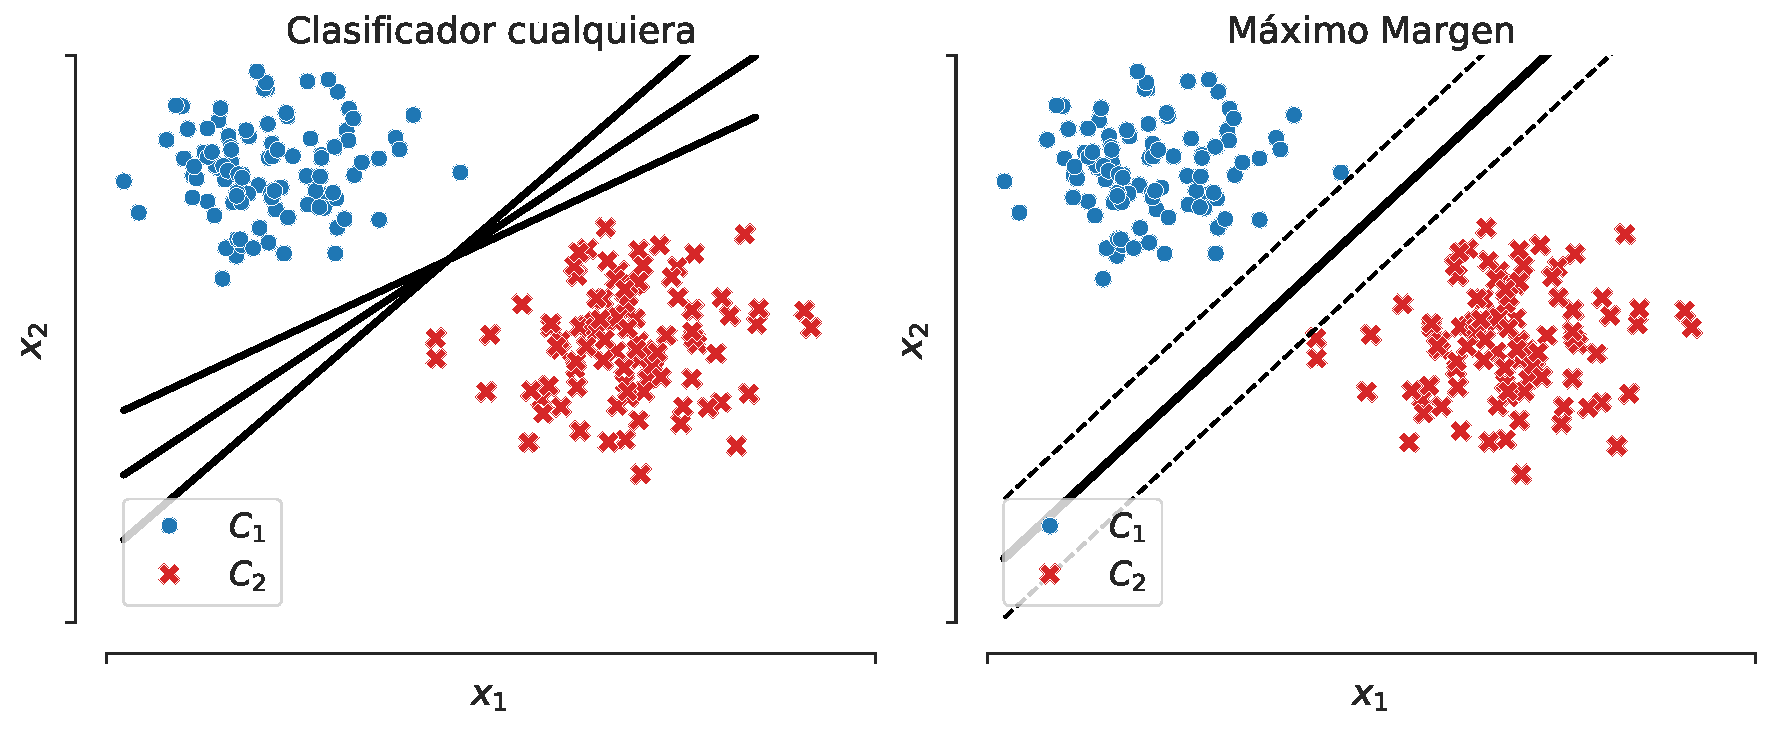
\includegraphics[width=0.9\textwidth]{../img/cap5_max_margen.pdf}
\end{figure}\pause

SVM busca el hiperplano separador que maximice el margen entre las clases, lo cual es equivalente a buscar una cinta de ancho máximo que separe los datos.
	
\end{frame}


%Ventajas de SVM
\begin{frame}{Ventajas de SVM}

Encontrar este clasificador tiene ventajas sobre los otros estudiados ya que:

\begin{itemize}
	\item Si los datos generados en cada clase provienen de una distribución latente, es de esperar que si se obtienen nuevos datos desde la misma distribución, estos estén cerca de los datos observados inicialmente. De este forma, SVM tiene buenas propiedades de generalización.\pause
	\item Como se verá a continuación, el clasificador de máximo margen queda definido únicamente por algunos datos. Esto inmediatamente resuelve el problema de desbalances de clase o de que las clases tengan formas distintas.\pause
	\item Por lo anterior, la solución de máximo margen se mantiene si agregamos datos que estén fuera del margen. Los datos que definen el margen los llamaremos vectores de soporte, cuya función será restringir la rotación y expansión del margen.
\end{itemize}
	
\end{frame}

%Formulación del problema: restricción sobre los vectores soporte.
\begin{frame}{Formulación del problema: restricción sobre los vectores soporte}

Dado un conjunto de entrenamiento $\{x_i\}_{i=1}^N$ linealmente separable, con clases $\{1,-1\}$, un hiperplano separador está definido mediante
\begin{equation*}
    \{x\in \R^n | w^\top x + b = 0 \}
\end{equation*}
Donde si $w^\top x + b >0$ se le asignará a $x$ la clase 1, mientras que si $w^\top x + b <0$ se le asignará a $x$ la clase -1.\\~\ \pause

El par $(w,b)$ no es único ya que si $(w,b)$ forma un hiperplano separador, entonces $(\lambda w, \lambda b)$ también lo hará.\\~\ \pause

Para evitar este escalamiento se impondrá una restricción sobre los bordes del margen. Sean $x_{+}$ y $x_{-}$ los vectores soporte de cada clase, se impone que estos pertenezcan a su respectiva clase, es decir:
\begin{align*}
 	w^\top x_{+} + b &= 1\\
 	w^\top x_{-} + b &=  -1,
 \end{align*}
 
 donde estos vectores soportes puede no ser únicos. Observemos que si bien aún no sabemos cuales son los vectores de soporte, podemos imponer esta restricción de todas formas.
 	
\end{frame}

%Formulación del problema: ancho del margen.
\begin{frame}{Formulación del problema: ancho del margen}

Las restricciones anteriores definen hiperplanos paralelos a la región de decisión ya que tienen el mismo parámetro $w$.\\~\ \pause

Por otro lado, el ancho del margen $m$, es la distancia entre la región de decisión y cualquiera de las clases.

\begin{columns}

\begin{column}{0.45\textwidth}
	\begin{figure}[ht]
    \centering
    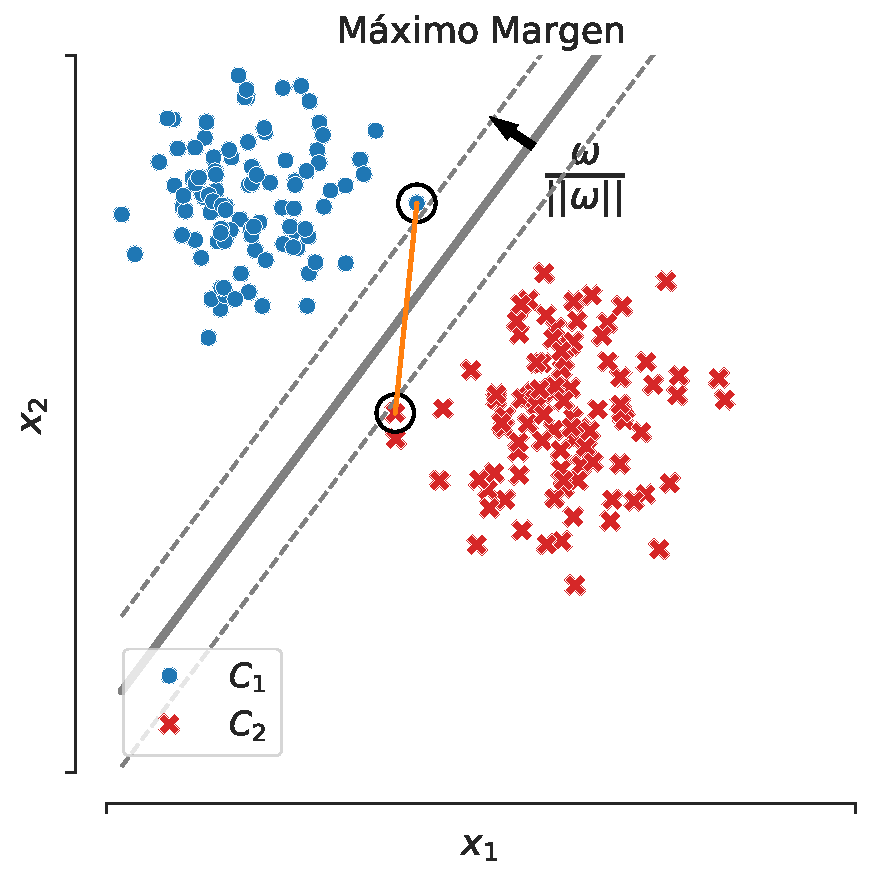
\includegraphics[width=\textwidth]{../img/cap5_max_margen2.pdf}
\end{figure}
\end{column}

\begin{column}{0.55\textwidth}\pause

En la figura se observa que el ancho del margen puede ser calculado como una proyección sobre la dirección normal del hiperplano, es decir, 
	\begin{align*}
m &= \frac{1}{2} \norm{\operatorfont{proy}_w(x_+-x_-)} \\
& =\frac{1}{2} \norm{x_+-x_-}\cos(\theta) \\
&= \frac{1}{2}\norm{x_+-x_-} \left(\frac{w^\top(x_+-x_-)}{\norm{w}\cdot\norm{x_+-x_-}}\right)\\
& =\frac{1}{2\norm{w}} w^\top(x_+ - x_-)
\end{align*}

\end{column}

\end{columns}

Donde se usó el hecho de que $\cos\left(\measuredangle(x,y)\right) = \frac{\langle x,y\rangle}{\norm{x}\norm{y}}$.
	
\end{frame}

%Formulación del problema: problema de optimización.
\begin{frame}{Formulación del problema: problema de optimización}

Además, el ancho del margen $m$ no depende explícitamente de los vectores soporte:
\begin{align*}
    m &= \frac{1}{2||w||} \left( (w^\top x_{+}) - (w^\top x_{-})\right)
    = \frac{1}{2||w||} \left((1-b) - (-1-b)\right)
    = \frac{1}{||w||}
\end{align*}\pause
Por otra parte, se considerará la siguiente codificación para las clases:
\begin{alignat*}{3}
    y_i&=+1 &&\Leftrightarrow w^\top x_i + b \geq +1 \\
    y_i &=-1 &&\Leftrightarrow w^\top x_i + b \leq -1
 \end{alignat*}\pause
 
Por lo tanto, se puede formular el problema de clasificación de máximo margen mediante el siguiente problema de optimización:
\begin{equation*}
\begin{aligned}
& \underset{w,b}{\text{max}}
& & \frac{1}{||w||}\\
& \text{s.a}
& & y_i (w^\top x_i +b) \geq 1, \; i = 1, \ldots, N.
\end{aligned}
\end{equation*}

Donde las restricciones exigen que todas las muestras sean bien clasificadas.
	
\end{frame}


%Formulación del problema: problema dual.
\begin{frame}{Formulación del problema: problema dual}

Para evitar problemas de diferenciablidad, se considerará la siguiente formulación equivalente del problema anterior:
\begin{equation*}
\begin{aligned}
(P)\quad & \underset{w,b}{\min}
& & \frac{1}{2}||w||^2\\
& \text{s.a}
& & y_i (w^\top x_i +b) \geq 1, \; i = 1, \ldots, N.
\end{aligned}
\end{equation*}\pause

Este problema de optimización con restricciones puede ser resuelto mediante dualidad lagrangiana:
\begin{equation*}
    L(w,b,\alpha) = \frac{1}{2}||w||^2 + \sum\limits_{i=1}^{N} \alpha_i \left(1-y_i (w^\top x_i +b)\right)
\end{equation*}\pause
	
El lagrangiano dual del problema viene dado por $\theta(\alpha) = \inf\limits_{w,b} L(w,b,\alpha)$ y dado que $L$ es convexo, basta aplicar la condición de primer orden:
\begin{align*}
	&\frac{\partial L}{\partial w} = w^\top - \sum_{i=1}^N \alpha_i y_i x_i^\top = 0 \implies \overline{w} = \sum_{i=1}^N \alpha_i y_i x_i\\
	&\frac{\partial L}{\partial b} = -\sum_{i=1}^N \alpha_i y_i = 0 \implies \sum_{i=1}^N \alpha_i y_i = 0
\end{align*}

	
\end{frame}


%Formulación del problema: problema final.
\begin{frame}{Formulación del problema: problema final}

Sustituyendo en $L$ y simplificando, el lagrangiano dual tiene la siguiente forma:

\begin{equation*}
	\theta(\alpha) = \frac{1}{2} \sum_{i,j=1}^N \alpha_i y_i \alpha_j y_j \langle x_i,x_j\rangle + \sum_{i=1}^N \alpha_i - \sum_{i,j=1}^N \alpha_i y_i \alpha_j y_j \langle x_j,x_i\rangle = \sum_{i=1}^N \alpha_i - \frac{1}{2} \sum_{i,j=1}^N \alpha_i \alpha_j y_i y_j \langle x_i,x_j\rangle
\end{equation*}\pause

Finalmente, el problema dual consiste en maximizar $\theta(\alpha)$ sujeto a que $\alpha\geq 0$, es decir:


\begin{equation*}
\begin{aligned}
(D)\quad & \underset{\alpha}{\max}
& & \sum\limits_{i=1}^{N}\alpha_i - \frac{1}{2} \sum\limits_{i,j=1}^{N} \alpha_i \alpha_j y_i y_j \langle x_i, x_j\rangle\\
& \text{s.a}
& & \sum\limits_{i=1}^{N} \alpha_i y_i= 0 \\
& &  &\alpha_i \geq 0
\end{aligned}
\end{equation*}

Donde la primera restricción se heredó de la CPO impuesta sobre $L$ al calcular $\theta(\alpha)$.
	
\end{frame}

%Observaciones de la formulación.
\begin{frame}{Observaciones de la formulación}

La forma usual para resolver SVM es mediante la resolución de su problema dual. Para este problema se tienen las siguientes observaciones:

\begin{itemize}
	\item La función objetivo es una forma cuadrática definida negativa.\pause
	\item Lo anterior implica que el problema tiene un único máximo.\pause
	\item Una vez resuelta la formulación dual (i.e., se han encontrado los valores óptimos para $\alpha$), la predicción de un nuevo punto $x_\star$ es de la forma 
\begin{equation*}
 	\hat{y}(x_\star)= \text{sgn} (\overline{w}^\top x_\star + b) = \text{sgn}\left(\left[\sum\limits_{i=1}^{N} \alpha_i y_i \langle x_i, x_\star\rangle\right] + b\right),
 \end{equation*}\pause
 
\item Por el teorema de holgura complementaria, para $\alpha$ óptimo se tiene que
\begin{equation*}
	\alpha_i \left(1-y_i (\overline{w}^\top x_i +b)\right) = 0,\quad \forall i\in\{1,\ldots,N\}
\end{equation*}
Por lo que $\alpha_i=0$ para todo $x_i$ fuera del margen y, consecuentemente, $x_i$ no aporta en la predicción $\hat{y}$.

\end{itemize}
	
\end{frame}

%Problemas del planteamiento anterior.
\begin{frame}{Problemas del planteamiento anterior}

El planteamiento anterior tiene dos debilidades:

\begin{itemize}
	\item Los datos no siempre serán separables por lo que el problema puede ser infactible.\pause
	\item Incluso si los datos son linealmente separables, el clasificador puede ser muy sensible a nuevos datos. Esto se observa en la siguiente figura:
\end{itemize}

\begin{figure}[ht]
    \centering
    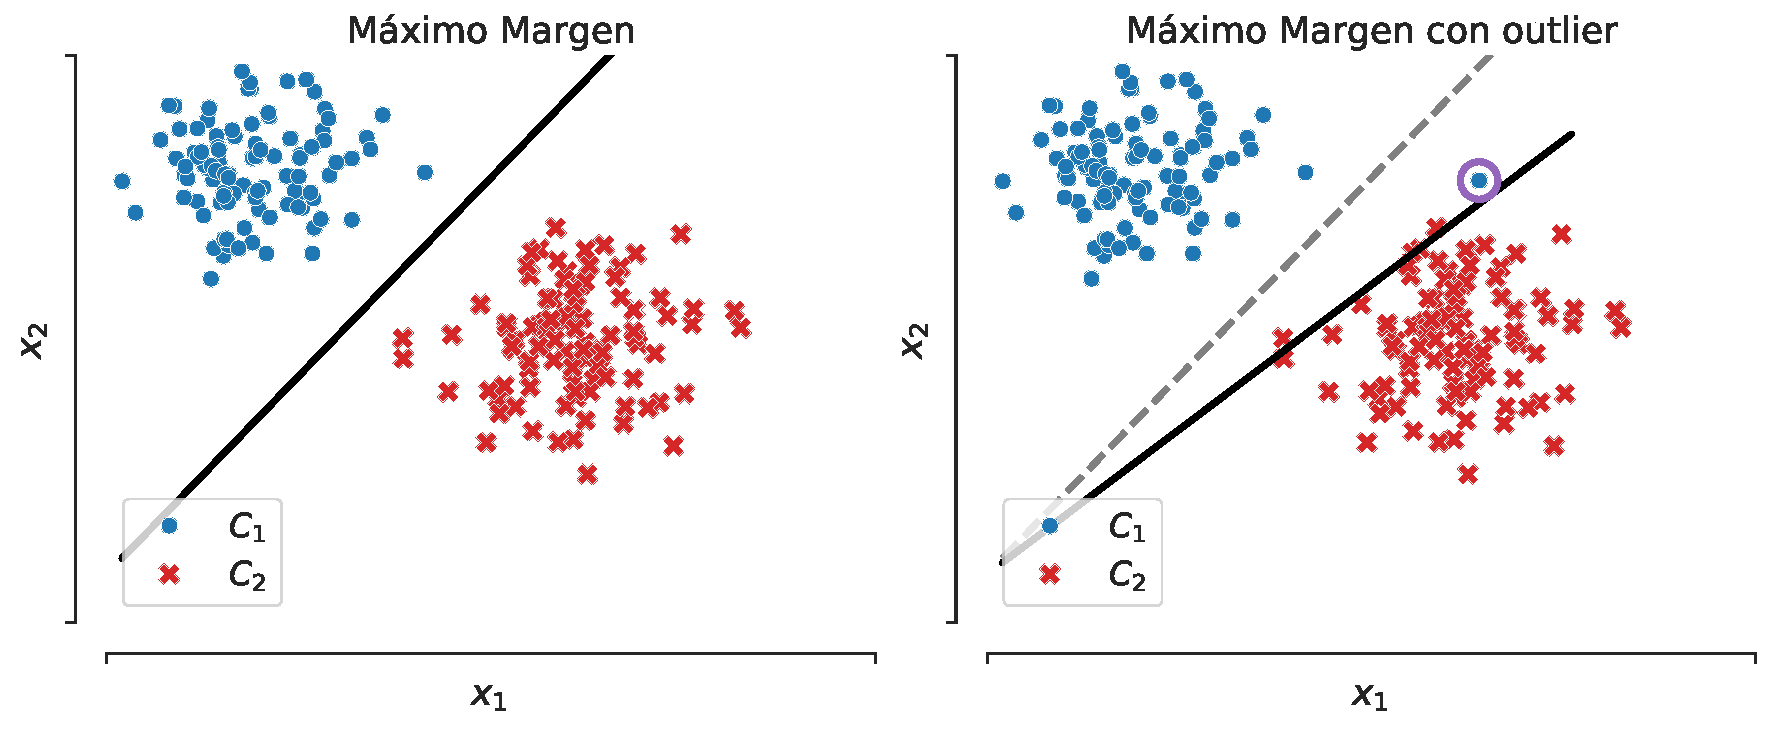
\includegraphics[width=0.9\textwidth]{../img/cap5_margen_suave}

\end{figure}

\end{frame}

%Margen suave: variables de holgura.
\begin{frame}{Margen suave: variables de holgura}

Para corregir las debilidades anteriores, se pueden introducir ``variables de holgura'', las cuales tienen el objetivo de permitir al clasificador admitir algunos datos incorrectamente clasificados.\\ \pause

\begin{columns}

\begin{column}{0.5\textwidth}
	\begin{figure}[ht]
    \centering
    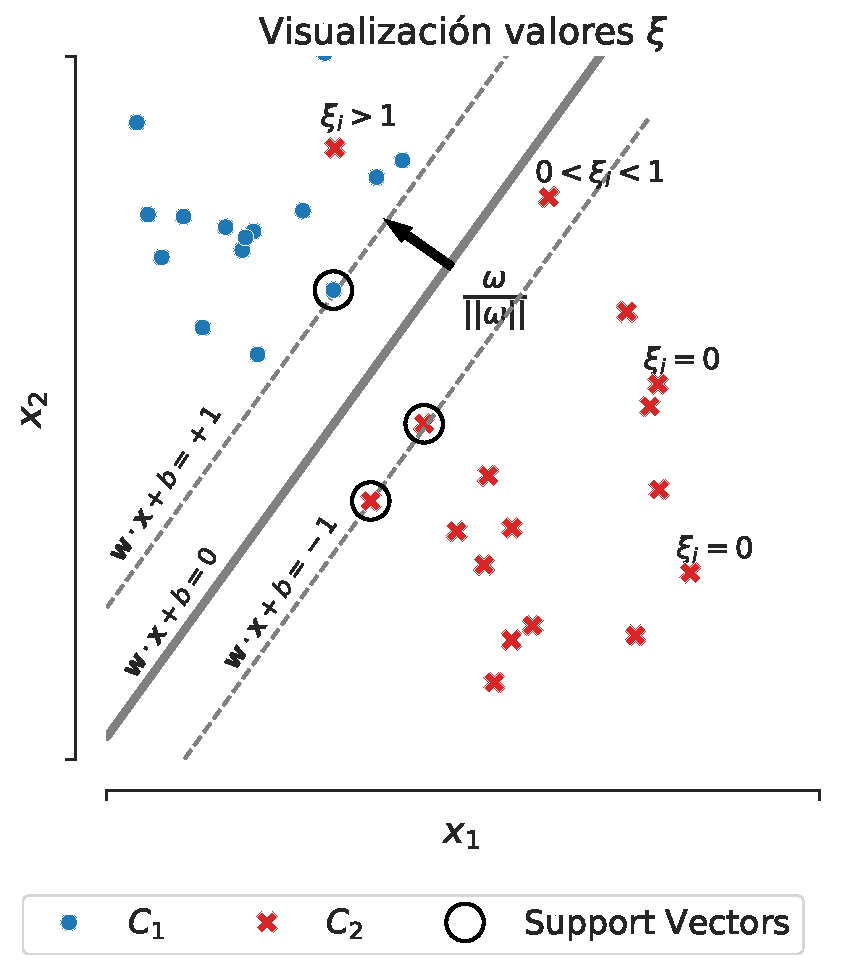
\includegraphics[width=1\textwidth]{../img/cap5_max_margen3}
\end{figure}
\end{column}

\begin{column}{0.5\textwidth}
	La formulación que \emph{perdona} algunos datos mal clasificados mediante la utilización de variables de holgura $\{\xi_i\}_{i=1}^N$ es la siguiente:

\begin{equation*}
\begin{aligned}
(P)\quad & \underset{w,b, \xi}{\text{min}}
& & \frac{1}{2}||w||^2 + c\sum\limits_{i=1}^{N} \xi_i \\
& \text{s.a}
& & y_i (w\cdot x_i +b) \geq 1 - \xi_i,\;\xi_i\geq0
\end{aligned}
\end{equation*}

donde $c>0$ es un hiperparámetro.\\ \pause

Se observa que la introducción del término $c\sum_{i=1}^{N} \xi_i$ en la función de costo puede ser interpretada como una regularización al igual que en MCR.

\end{column}

\end{columns}

\end{frame}

%Margen suave: formulación.
\begin{frame}{Margen suave: formulación}

Procediendo de la misma forma que en el caso anterior, el dual de este problema es:
\begin{equation*}
\begin{aligned}
(D)\quad & \underset{\alpha}{\text{max}}
& & \sum\limits_{i=1}^{N}\alpha_i - \frac{1}{2} \sum\limits_{i,j=1}^{N} \alpha_i \alpha_j y_i y_j \langle x_i, x_j\rangle\\
& \text{s.a}
& & \sum\limits_{i=1}^{N} \alpha_i y_i= 0 \\
& &  &0 \leq \alpha_i \leq c.
\end{aligned}
\end{equation*}\pause

Se observa que:

\begin{itemize}
	\item La diferencia entre ambas formulaciones está dada por el hecho de que los multiplicadores de Lagrange ahora están acotados por el hiperparámetro $c$.\pause
	\item $c$ representa la importancia que se da a la suma de las variables de holgura versus el ancho del margen.\pause
	\item Cuando $c\to\infty$ se recupera la formulación original (margen duro).\pause
	\item La elección de este hiperparámetro puede realizarse mediante validación cruzada.
\end{itemize}

\end{frame}

\end{document}
